\chapter{API REST: interface technique du Portail Pro}

\section{Introduction}
Pour les organisations qui utilisent un logiciel de gestion des activités accueil temps libre (présences des enfants, des encadrants, etc.), l'ONE met à disposition une Application Programming Interface (API REST) permettant de faire transiter des données de manière sécurisée depuis votre logiciel vers le Portail Pro.one.be. 

Cette connexion vous demandera certainement des efforts de développement. Renseignez-vous auprès de votre fournisseur de logiciel pour évaluer la plus-value de ce développement.

Vous pouvez fournir à vos développeurs (ou à votre fournisseur de logiciel) le lien vers la documentation technique que vous trouverez au point \ref{api_doc}.

Pour le moment, l'API REST est disponible pour le secteur des Centres de vacances (\ref{api:cdv}) et pour le secteur de l'Accueil extrascolaire (type 1) (point \ref{api:aes1}). 


Notez que l'API REST Centres de vacances est construit pour le moment pour recevoir les déclarations et demandes de subvention pour les camps de vacances des mouvements de jeunesse. Si vous souhaitez utiliser l'API REST pour vos plaines ou séjours, prenez contact avec l'ONE.




\section{Documentations techniques (lien)}\label{api_doc}
La documentation technique permet à l'équipe de développement de prendre connaissance des spécificités techniques à développer pour la transmission des données. \textbf{Lien vers la documentation technique}: 

\url{https://pro-atl.one.be/swagger-ui/index.html?configUrl=\%2Fv3\%2Fapi-docs\%2Fswagger-config}



\section{Utilisateur technique}\label{api:user}
Une fois que votre système a été adapté, il sera nécessaire d'utiliser un identifiant technique pour vous identifier. Cet identifiant sera nécessaire pour que votre API REST puisse fonctionner et envoyer les données vers le Portail Pro.one.be.

\subsection{Créer un utilisateur technique}
La création de cet identifiant se fait dans le panel d'administration > Applications externes. Vous retrouverez la liste des identifiants techniques de votre organisation (Voir fig. \ref{subfig:create_user}).

Pour créer un utilisateur technique, cliquez sur \ovalbox{Ajouter un utilisateur technique}. Vous serez invité à créer un nom d'utilisateur. Le mot de passe est quant à lui généré de manière aléatoire par le système. Cliquez sur \ovalbox{Ajouter l'utilisateur}. (Voir fig. \ref{subfig:add_user}). 



\begin{figure}[!h]
    \centering
    \begin{subfigure}[t]{0.48\textwidth}
         \centering
         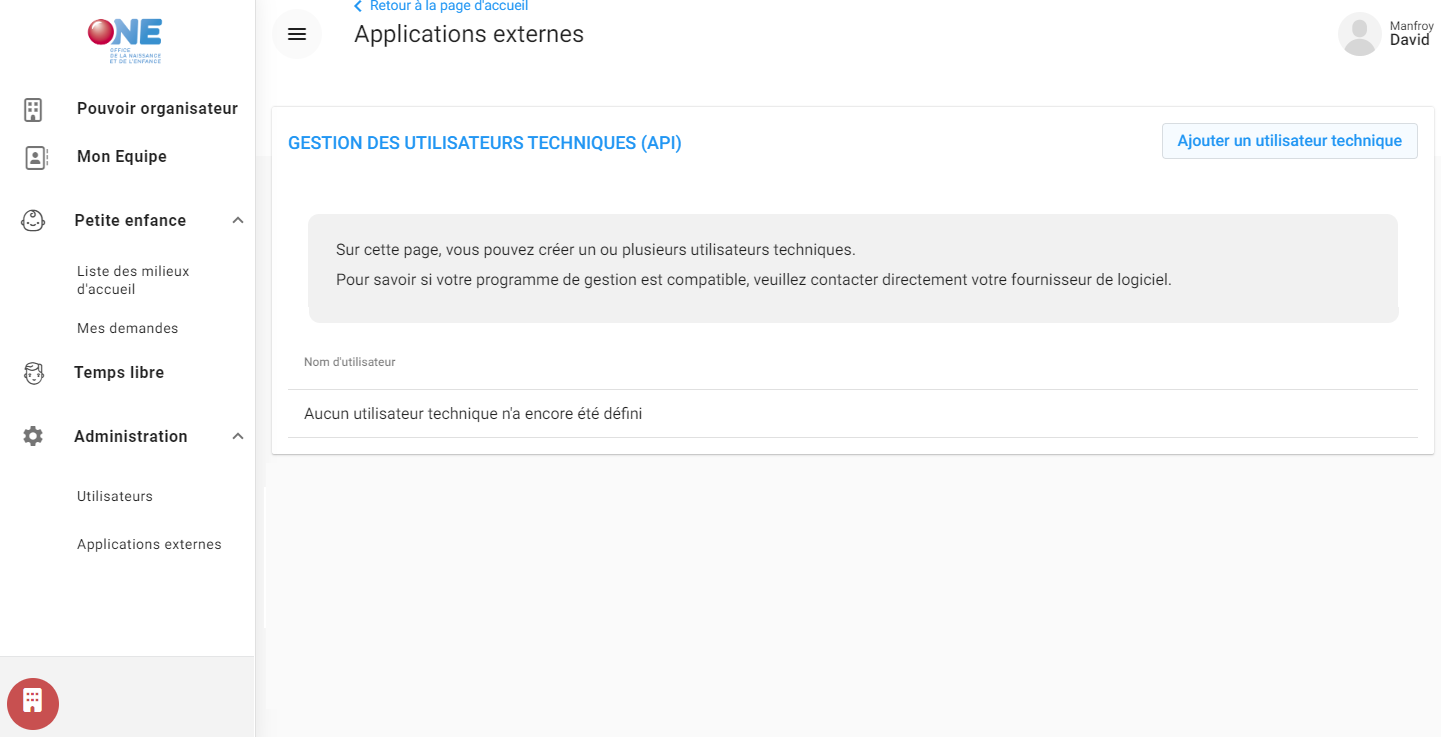
\includegraphics[width=0.95\textwidth, frame]{Images/api/create_user.png}
         \caption{Liste des utilisateurs techniques pour l'utilisation d'API REST du Portail Pro.one.be}
         \label{subfig:create_user}
     \end{subfigure}
     %\hfill
    \begin{subfigure}[t]{0.48\textwidth}
         \centering
         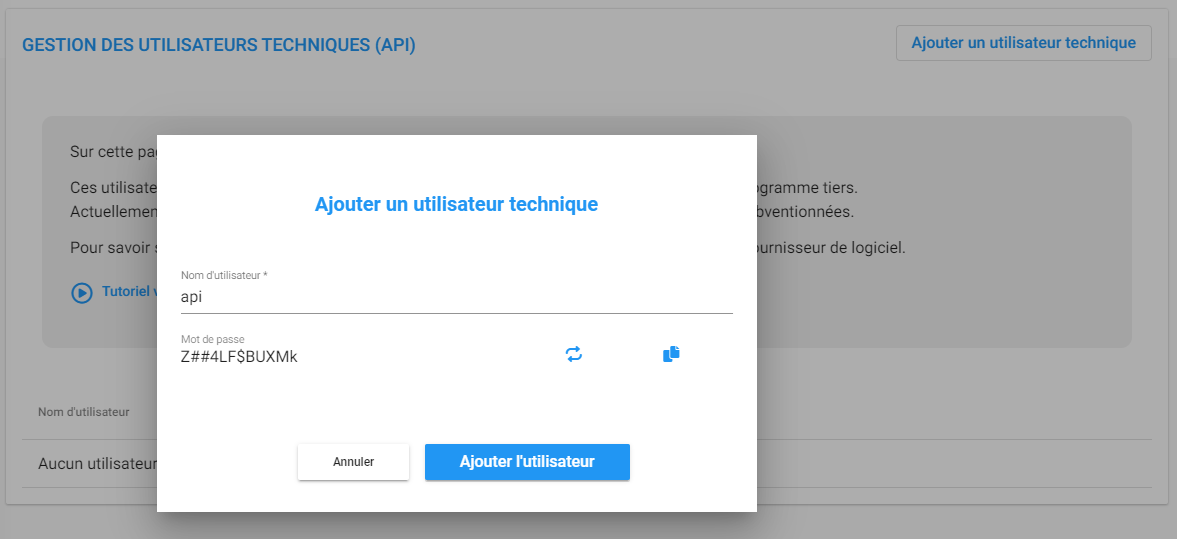
\includegraphics[width=0.95\textwidth, frame]{Images/api/add_user.png}
         \caption{Ajout d'un nouvel utilisateur technique}
         \label{subfig:add_user}
     \end{subfigure}

    
    \caption{L'entrée Utilisateurs techniques vous permet de créer, configurer ou supprimer des identifiants nécessaires pour l'utilisation d'API REST.}
    \label{fig:user_technique}
    
\end{figure}

\subsection{Configurer les droits d'accès de  l'utilisateur technique}

Pour l'Accueil Temps Libre, vous pouvez configurer l'accès pour que l'utilisateur puisse utiliser l'API Centres de vacances ou l'API Accueil extrascolaire en cliquant sur le petit crayon. Cochez ensuite les secteurs dont vous souhaitez octroyer les accès (voir fig.\ref{fig:config_user}). 

Si votre application ne gérera que la transmission des données Accueil extrascolaire, mais pas Centres de vacances, nous vous conseillons de limiter les accès qu'au secteur concerné pour des questions de sécurité en décochant les cases concernées.

\begin{figure}[h!]
    \centering
    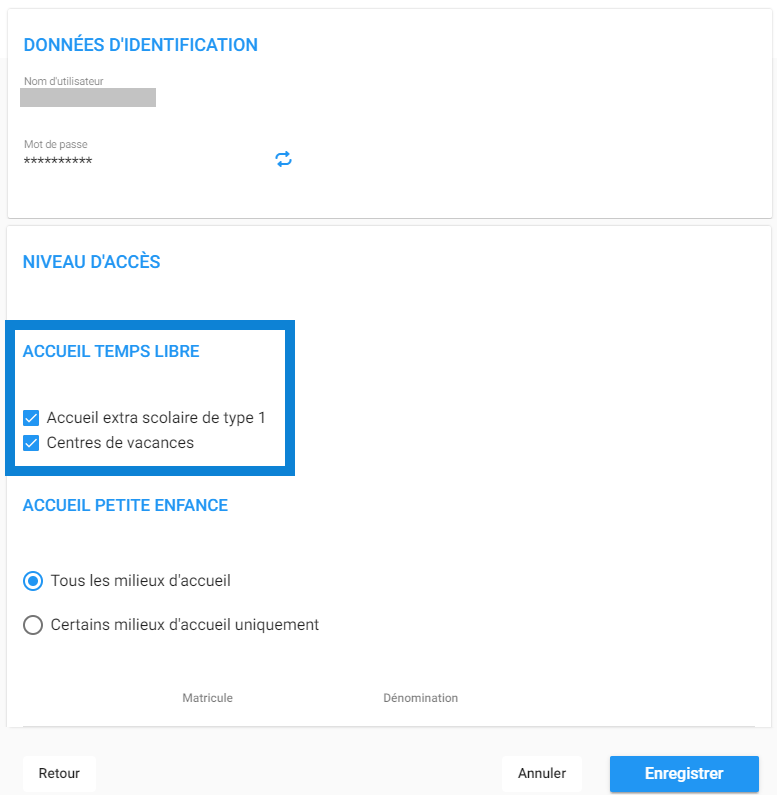
\includegraphics[width=7cm,frame]{Images/api/config_user.png}
    \caption{Configuration des utilisateurs techniques.}
    \label{fig:config_user}
\end{figure}

\subsection{Renouveler le mot de passe technique}
Pour renouveler le mot de passe de l'utilisateur technique, vous pouvez cliquez sur le petit crayon de modification. L'icône 
\includegraphics[width=0.35cm]{Images/icon/button_renew_mdp.png} vous permettra de générer un nouveau mot de passe aléatoire. 

N'oubliez pas de configurer votre logiciel avec ce nouveau mot de passe pour que l'authentification puisse se réaliser. Sans cette nouvelle configuration, votre logiciel ne pourra pas envoyer de données vers le Portail Pro.one.be. Demandez à votre fournisseur de logiciel la manière dont l'authentification technique est réalisée et où la configuration se réalise. 

\subsection{Supprimer un utilisateur technique}
Si vous n'utilisez plus l'utilisateur technique d'API, nous vous conseillons fortement de le supprimer. En effet, ces utilisateurs techniques pour des questions évidente de sécurité d'accès. La suppression se réalise en cliquant sur la 
\includegraphics[width=0.35cm]{Images/icon/button_poubelle_api.png}. 



\section{API - Accueil Temps Libre}\label{api:atl}

\subsection{Modification du contact général}
Cet API permet de modifier le contact général de votre Pouvoir organisateur (voir fig.\ref{fig:general_contact}).

\begin{figure}[h!]
    \centering
    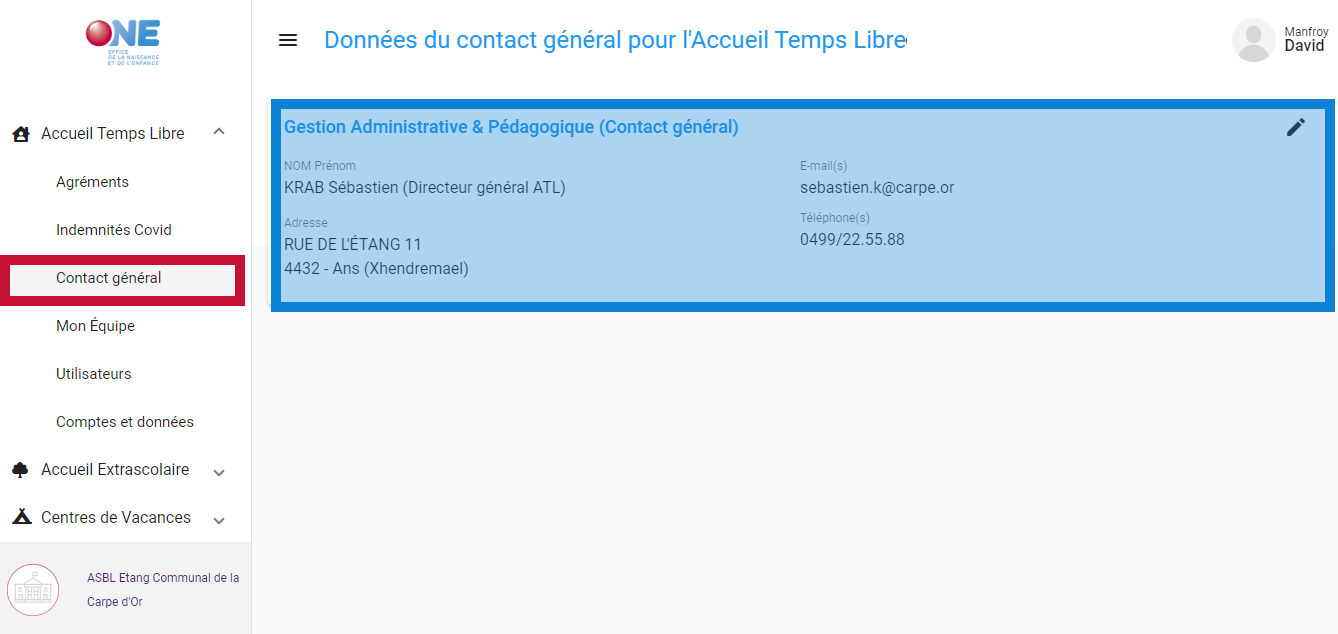
\includegraphics[width=9cm,frame]{Images/api/general_contact.png}
    \caption{Dans l'application, le contact général est la personne de contact principal de votre Pouvoir organisateur.}
    \label{fig:general_contact}
\end{figure}



\subsection{Gestion du personnel d'encadrement}
Cet API permet de déclarer du personnel au niveau de votre Pouvoir organisateur dans "Mon Équipe" et de déposer des informations de brevet uniquement.

N'est pas pris en charge via l'API le fait d'assigner les personnes à un secteur donnée en ATL (Centres de vacances ou Accueil extrascolaire) et le fait de les assigner à un lieu d'accueil extrascolaire ou une activité centres de vacances. 
N'est pas pris en charge non plus les créations de contrat de travail. 


\section{API - Centres de vacances}\label{api:cdv}
\subsection{Préambule - API REST orienté camp de vacances}
L'API pour les Centres de vacances a été développée initialement pour les Fédération de Mouvement de jeunesse (Les Scouts, Les Guides de Belgique, La Fédération nationale des Patros, Les Scouts et Guides Pluraliste (SGP), Les Faucons Rouges). 

Si vous êtes un Pouvoir organisateur de Plaine ou de séjour de vacances, vous pourrez utiliser sans inconvénient les API de :
\begin{itemize}
    \item Modification du contact Centres de vacances (point \ref{api:contact_cdv});
    \item Déclaration d'activité Centres de vacances (point \ref{api:da_cdv}). 
\end{itemize}

Par contre, l'API de déclaration de présences (\ref{api:ds_cdv_présences}) pour les activités qui présentent des encadrants indemnisés ne pourront pas répondre à votre besoin pour le moment. Pour qu'on puisse étudier votre besoin, contactez l'ONE. 


\subsection{Contact Centres de vacances}\label{api:contact_cdv}
Cette API permet de mettre à jour la personne de contact pour le secteur des centres de vacances. Ces informations de contact seront utilisées par l'ONE pour toutes les questions relatives à l'organisation de vos Centres de vacances (gestion des dossiers, déclaration d'activité, demande de subvention, décision sur la demande de subvention, recours, etc). 


\subsection{Déclaration d'activité}\label{api:da_cdv}
Cette API permet de déclarer vos activités de Centres de vacances. 

\subsection{Demande de subvention}\label{api:ds_cdv}

\subsubsection{Déclaration d'enfants}\label{api:ds_cdv_enfants}
Cette API permet la récupération et la déclaration des données de fréquentation des enfants de l'activité centres de vacances. 

\subsubsection{Déclaration de présences}\label{api:ds_cdv_présences}
Cette API permet la récupération et la déclaration des présences (enfants et encadrants) d'une activité centres de vacances. Les présences des encadrants ne sont possibles uniquement pour les animateurs et animateur-responsable qui sont volontaires non-indemnisés (camp de mouvement de jeunesse)

\begin{attention}
Les présences des encadrants indemnisés (contrat de travail, étudiants, etc.) ne pourront pas être déclarés via l'API. La version actuelle de l'API REST n'est utilisable que pour les encadrants de mouvement de jeunesse (volontaire non-indemnisés). 
\end{attention}


\subsubsection{Envoie de la demande de subvention}
L'introduction d'une demande de subvention n’est possible qu’une fois les critères suivants rencontrés :
\begin{itemize}
    \item l'activité est terminée,
    \item le personnel d'encadrement a été déclaré, 
    \item les présences (enfants et encadrants) ont été déclarées, 
    \item les données de fréquentation ont été communiquées, 
\end{itemize}






\section{API - Accueil extrascolaire}\label{api:aes1}

\subsection{Lieux d'accueil extrascolaire}
Cette API permet de récupérer les données des lieux d'accueil extrascolaire du pouvoir organisateur. 


\subsection{Fréquentations}
Permet de récupérer et de déclarer les données de fréquentation d'un lieu d'accueil extrascolaire pour un trimestre donné. Pour déclarer des données de fréquentations, l'utilisateur doit avoir préalablement mis à jour les horaires d'accueil de l'année concernée. Le point \ref{subsec:aes_horaire} du chapitre "Accueil extrascolaire" vous donnera les démarches à effectuer via le Portail Pro.one.be (fig. \ref{fig:api_aes_horaires}).

\begin{figure}[htbp]
    \centering
    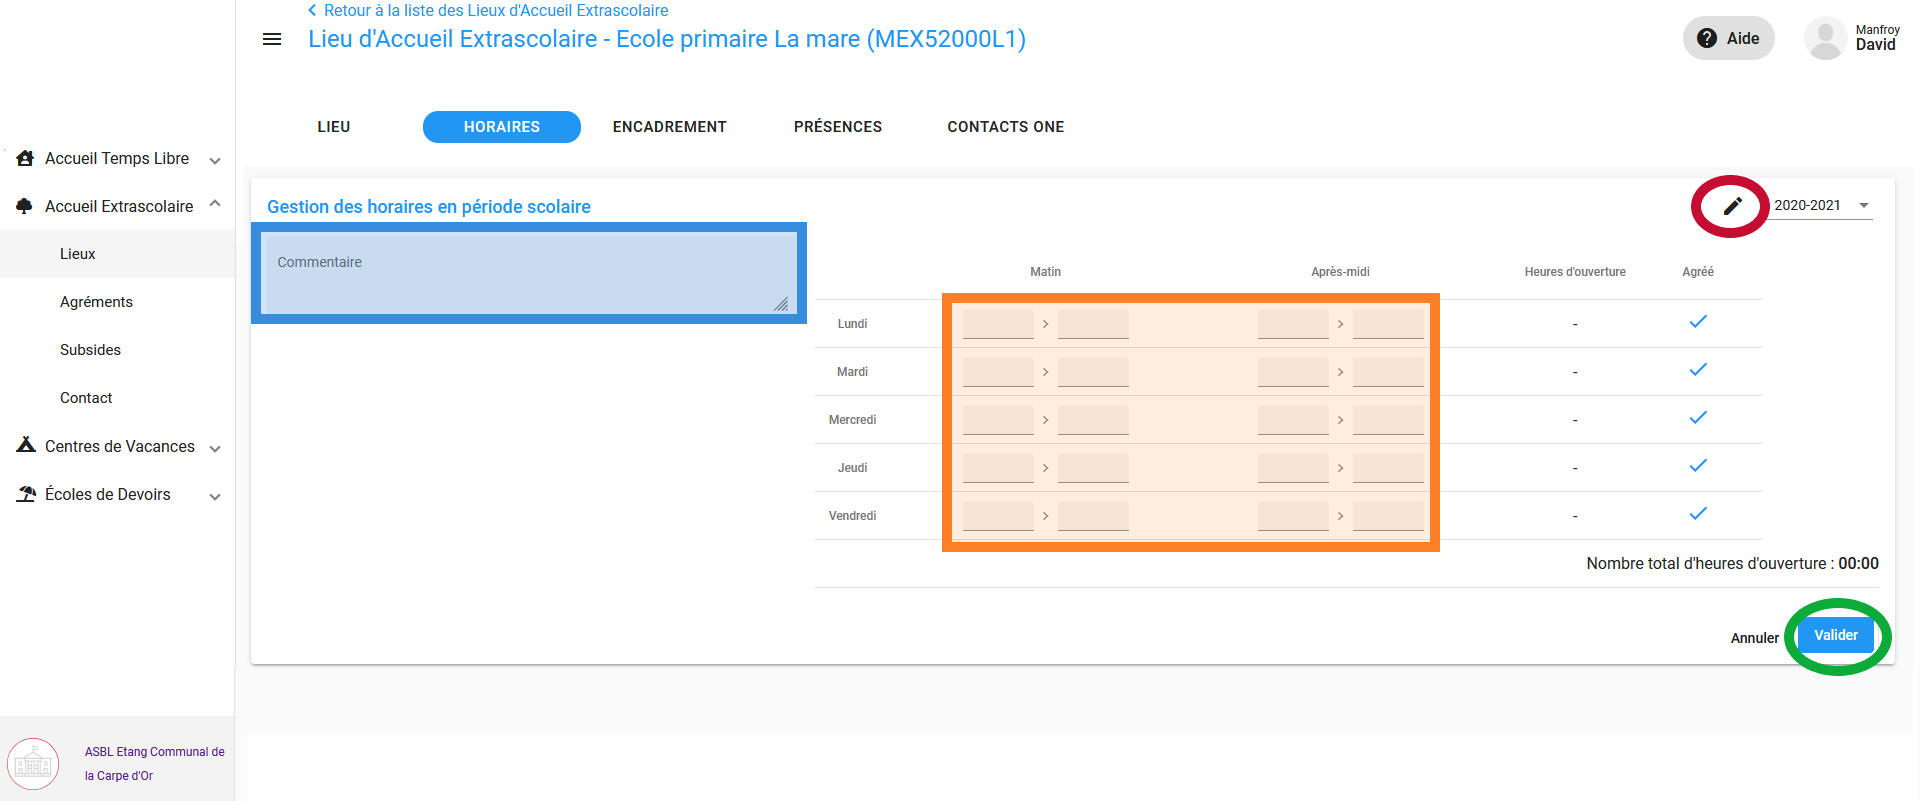
\includegraphics[width=15cm]{Images/aes/horaire2.png}
    \caption{Pour utiliser l'API REST, il sera nécessaire de compléter préalablement l'onglet horaires dans la web-app.}
    \label{fig:api_aes_horaires}
\end{figure}




\subsection{Présences}
Permet la récupération et la déclaration des présences enfants d'un lieu d'accueil extrascolaire pour un mois donné. La déclaration/mise à jour de présences n'est possible qu’une fois les critères suivants rencontrés :
\begin{itemize}
    \item le lieu d'accueil extrascolaire prévoit l'accueil d'enfants issus de la maternelle et/ou du primaire, voir /api/aes1/places (donnée modifiable uniquement via la webapp) (voir le point \ref{ssec:aes_lieu});
    \item l'horaire de l'année scolaire a été encodé pour le lieu (donnée consultable et modifiable uniquement via la webapp) (fig. \ref{fig:api_aes_horaires});
    \item les données de fréquentation du trimestre ont été déclarées pour le lieu.
\end{itemize}   

Il sera nécessaire de se connecter au Portail Pro (webapp) et mettre à jour l'horaire de l'année et, si nécessaire, les caractéristiques d'accueil.



\subsection{Subventions}
Permet l'envoi d'une demande de subvention trimestrielle d'un lieu d'accueil extrascolaire. L'introduction d'une demande de subvention trimestrielle n’est possible qu’une fois les critères suivants rencontrés :

\begin{itemize}
    \item le trimestre est révolu;
    \item les présences ont été déclarées pour le trimestre et le lieu concernés.
\end{itemize}






